%! Author = gramic
%! Date = 29.02.24

% Preamble
%\begin{landscape}
\clearpage
\KOMAoptions{paper=A3,paper=landscape,pagesize,DIV=20}
\recalctypearea
%\begin{flushleft}
%\pagestyle{headings}
%    \clearpage
%    \KOMAoptions{paper=A3,paper=landscape,pagesize,DIV=20}
%    \recalctypearea
    \chapter{Projektmanagement}
    \section{Projektplanung}
    \subsection{Projektcontrolling}
    Die geleistete Arbeit und verbleibende Zeit wird in nachfolgender Tabelle gelistet:
    \begin{table}[H]

\resizebox{\columnwidth}{!}{%

\begin{tabular}{lllrrr}
\toprule
 & Phase & Subphase & Dauer [h] & Geplante Dauer [h] & Verbleibende Zeit [h] \\
\midrule
0 & 1. Expertengespräch & 1. Expertengespräch & 1.0 & 1.0 & 0.0 \\
1 & 2. Expertengespräch & 2. Expertengespräch & 1.2 & 1.0 & -0.2 \\
2 & Aufbau und Implementation Testsystem & Basisinfrastruktur & 3.0 & 4.0 & 1.0 \\
3 & Aufbau und Implementation Testsystem & Installation und Konfiguration PostgreSQL HA Cluster & 20.0 & 20.0 & 0.0 \\
4 & Aufbau und Implementation Testsystem & Technical Review & 2.0 & 3.0 & 1.0 \\
5 & Dokumentation & Dokumentation & 44.8 & 80.0 & 35.2 \\
6 & Evaluation & Analyse PostgreSQL HA Cluster Lösungen & 51.2 & 16.0 & -35.2 \\
7 & Evaluation & Anorderungskatalog & 4.5 & 16.0 & 11.5 \\
8 & Evaluation & Gegenüberstellung & 0.5 & 8.0 & 7.5 \\
9 & Evaluation & Variantenentscheid & 1.0 & 4.0 & 3.0 \\
10 & Evaluation & Vorbereitung Benchmarking & 5.0 & 4.0 & -1.0 \\
11 & Letztes Expertengespräch & Letztes Expertengespräch & 0.0 & 1.0 & 1.0 \\
12 & Puffer & Puffer & 0.0 & 16.0 & 16.0 \\
13 & Resultate & Persönliches Fazit & 0.0 & 2.0 & 2.0 \\
14 & Resultate & Schlussfolgerung & 0.0 & 2.0 & 2.0 \\
15 & Resultate & Weiteres Vorgehen / offene Arbeiten & 0.0 & 1.0 & 1.0 \\
16 & Resultate & Zielüberprüfung & 1.0 & 2.0 & 1.0 \\
17 & Testing & Protokollierung & 0.0 & 4.0 & 4.0 \\
18 & Testing & Review und Auswertung & 2.2 & 2.0 & -0.2 \\
19 & Testing & Testing Testsystem & 6.2 & 8.0 & 1.8 \\
20 & Troubleshooting und Lösungsfindung & Troubleshooting und Lösungsfindung & 11.0 & 8.0 & -3.0 \\
Total &  &  & 154.8 & 203.0 & 48.2 \\
\bottomrule
\end{tabular}
}
\caption{Projektcontrolling} \label{projektcontrolling}
\end{table}

%\end{flushleft}
%\clearpage
%\KOMAoptions{paper=A4,paper=portrait,pagesize}
%\recalctypearea
%\begin{flushleft}
%\clearpage
%\KOMAoptions{paper=A4,paper=portrait,pagesize}
%\recalctypearea
%\pagestyle{headings}
%%\begin{flushleft}
%%    \begin{figure}[H]
%%        \centering
%%        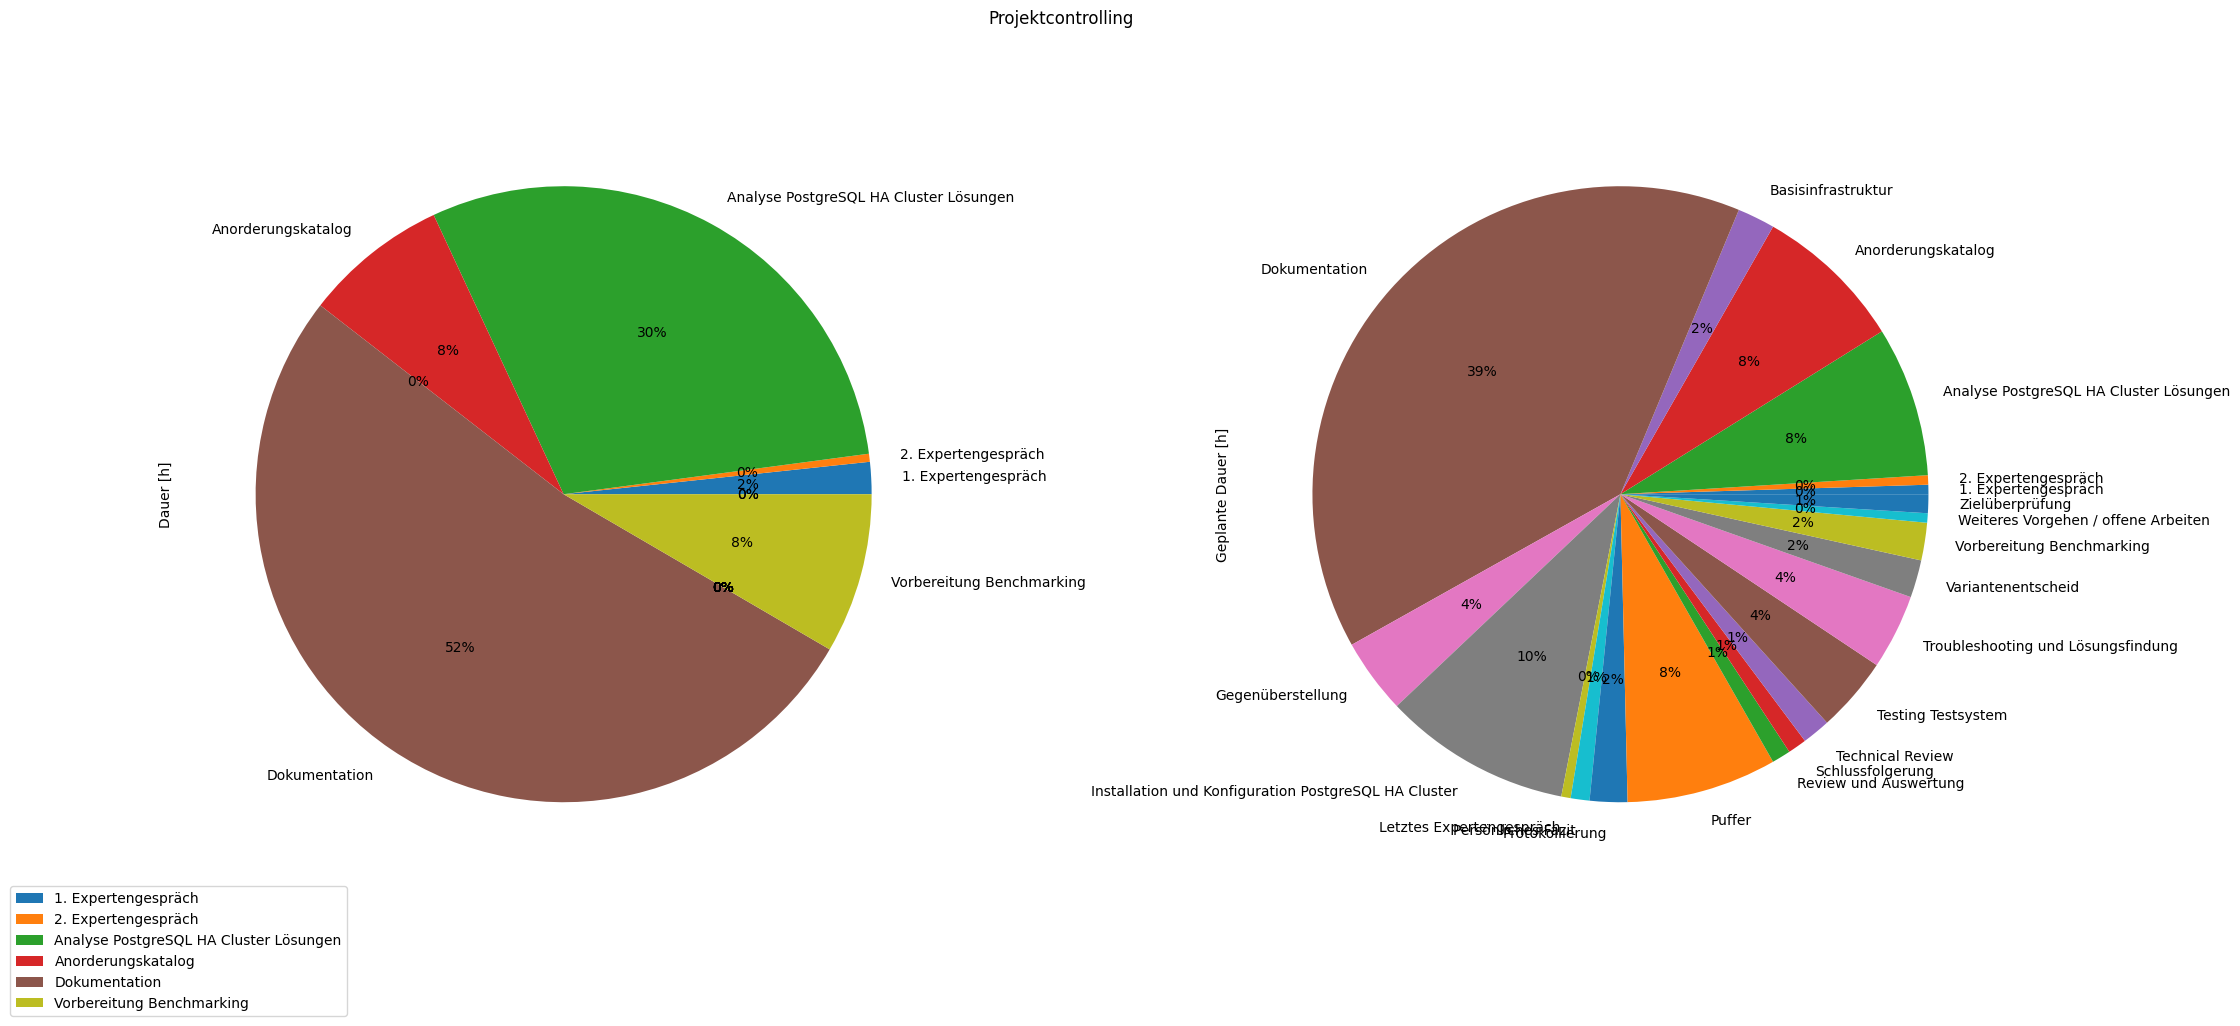
\includegraphics[width=0.75\linewidth]{source/pandas_data_chart_plotter/projektcontrolling}
%%        \caption{Projektcontrolling}
%%        \label{fig:projektcontrolling}
%%    \end{figure}
%    \begin{figure}[H]
%        \centering
%        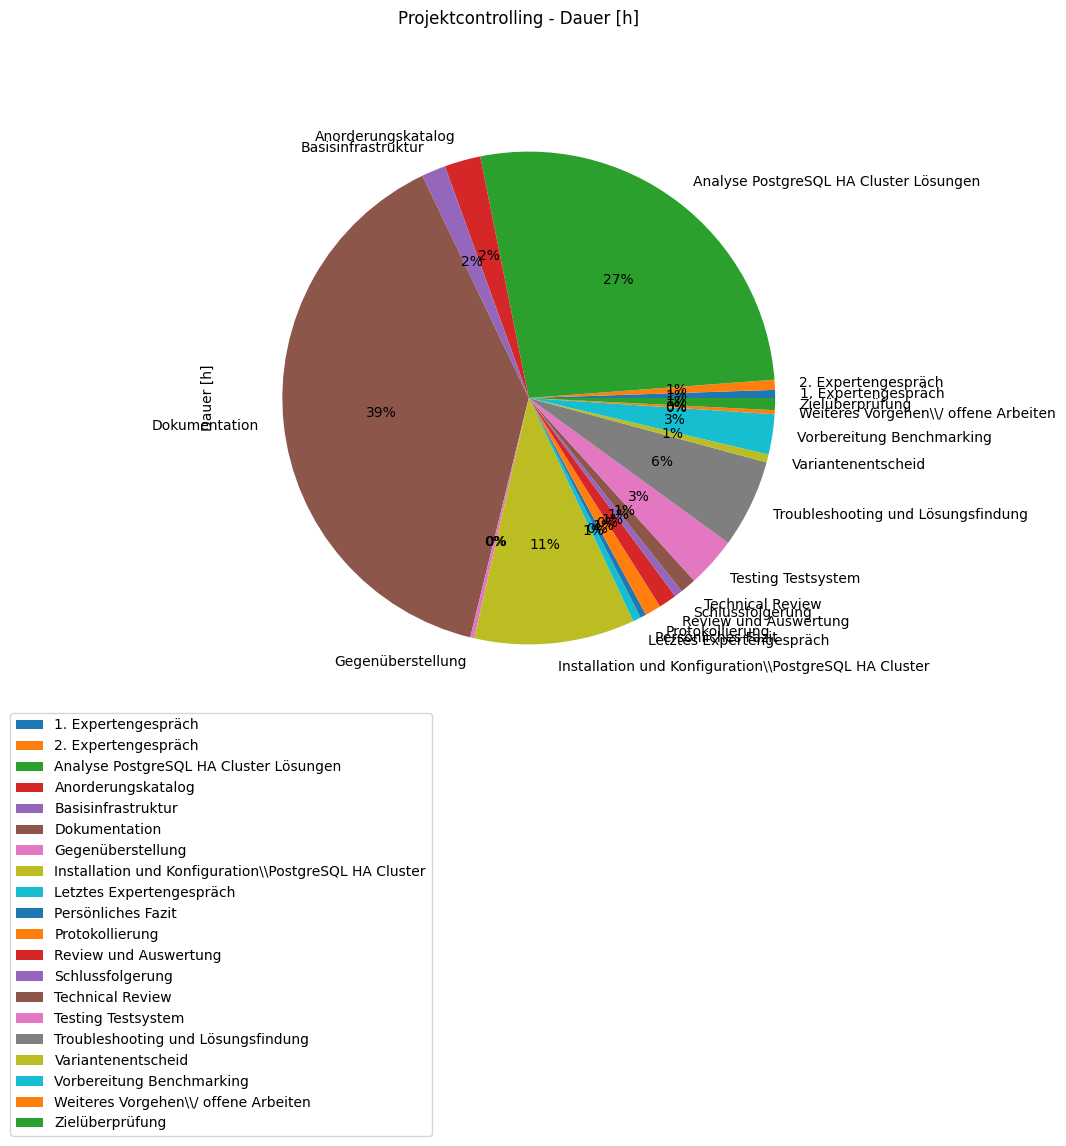
\includegraphics[width=0.75\linewidth]{source/pandas_data_chart_plotter/projektcontrolling_dauer}
%        \caption{Projektcontrolling - Dauer}
%        \label{fig:projektcontrolling_dauer}
%    \end{figure}
%\end{flushleft}
%\begin{flushleft}
%\clearpage
%\KOMAoptions{paper=A4,paper=portrait,pagesize}
%\recalctypearea
%    \begin{figure}[H]
%        \centering
%        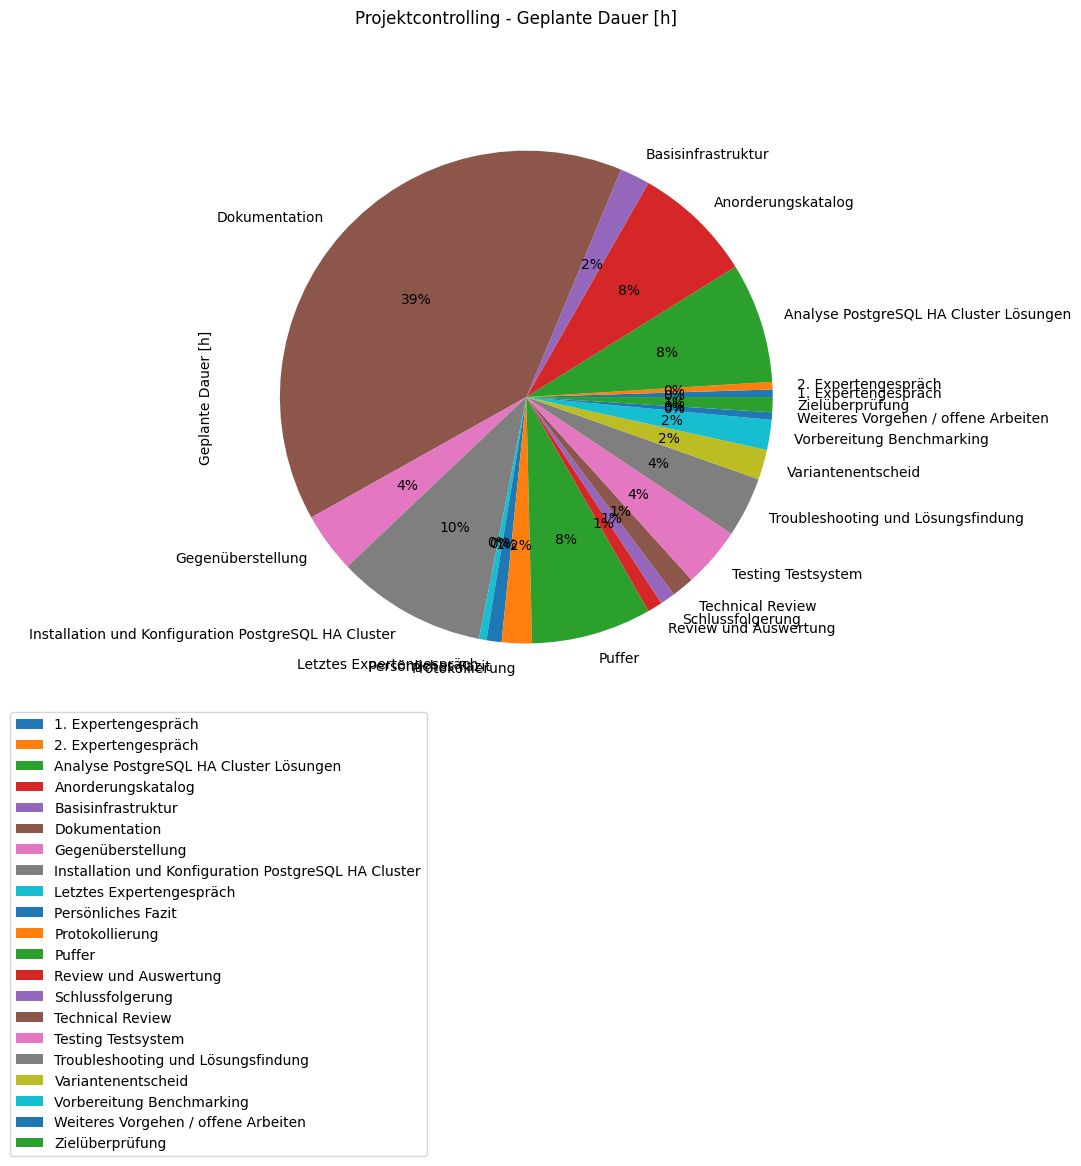
\includegraphics[width=0.75\linewidth]{source/pandas_data_chart_plotter/projektcontrolling_geplant}
%        \caption{Projektcontrolling - Geplante Dauer}
%        \label{fig:projektcontrolling_geplant}
%    \end{figure}
%\end{flushleft}
%\clearpage
%\end{landscape}